\documentclass[tikz,border=10pt]{standalone}
\begin{document}
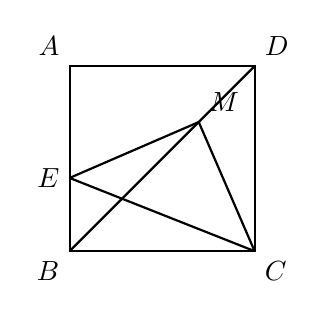
\begin{tikzpicture}[thick, scale=1]
  \coordinate (A) at (0,2.35);
  \coordinate (B) at (0,0);
  \coordinate (C) at (2.35,0);
  \coordinate (D) at (2.35,2.35);
  \coordinate (E) at (0,0.93);
  \coordinate (M) at (1.64,1.64);

  \draw (A) -- (D) -- (C) -- (B) -- cycle;
  \draw (B) -- (D);
  \draw (E) -- (M);
  \draw (M) -- (C);
  \draw (E) -- (C);

  \node[above left] at (A) {$A$};
  \node[above right] at (D) {$D$};
  \node[below left] at (B) {$B$};
  \node[below right] at (C) {$C$};
  \node[left] at (E) {$E$};
  \node[above right] at (M) {$M$};
\end{tikzpicture}
\end{document}
